
\documentclass[aspectratio=169,xcolor=dvipsnames]{beamer}
%\usetheme{SimplePlus}
\usepackage{hyperref}
\usepackage{graphicx} % Allows including images
\usepackage{booktabs} % Allows the use of \toprule, \midrule and \bottomrule in tables
\usepackage[utf8]{inputenc}
\usepackage[T1]{fontenc}

%----------------------------------------------------------------------------------------
%	TITLE PAGE
%----------------------------------------------------------------------------------------

\title[posisjon]{Måling av turtall og posisjon} % The short title appears at the bottom of every slide, the full title is only on the title page
%\subtitle{Subtitle}

\author[Fred-Olav] {Fred-Olav Mosdal}

\institute[Gand VGS] % Your institution as it will appear on the bottom of every slide, may be shorthand to save space
{
    Gand VGS \\
    VG3 Automasjon }
\date{\today} % Date, can be changed to a custom date


%----------------------------------------------------------------------------------------
%	PRESENTATION SLIDES
%----------------------------------------------------------------------------------------

\begin{document}
\begin{frame}
	\frametitle{Turtall og Posisjon}
	I automatiserte anlegg brukes roterende maskiner for å drive utstyr som pumper, vifter og transportbånd. 
	\vskip 0.5cm
	Ofte er de nyttig å vite hvor fort disse går. For transportbåndet kan det også være kjekt å vite hvor langt det har gått. 
	Til dette bruker vi posisjons- og hastighetsmåling. 
\end{frame}


\begin{frame}
	\frametitle{Enkodere}
	\begin{columns}
		\begin{column}{0.5\textwidth}
		\begin{itemize}
			\item Enkodere kan brukes til å måle turtall og posisjon
			\item Enkodere brukes ofte i servosystemer (reguleringssløyfe for posisjon/turtall)
				\item Enkodere fines i utgaver inkrementell- eller absolutt giver
		\end{itemize}	
		\end{column}

		\begin{column}{0.5\textwidth}
	$$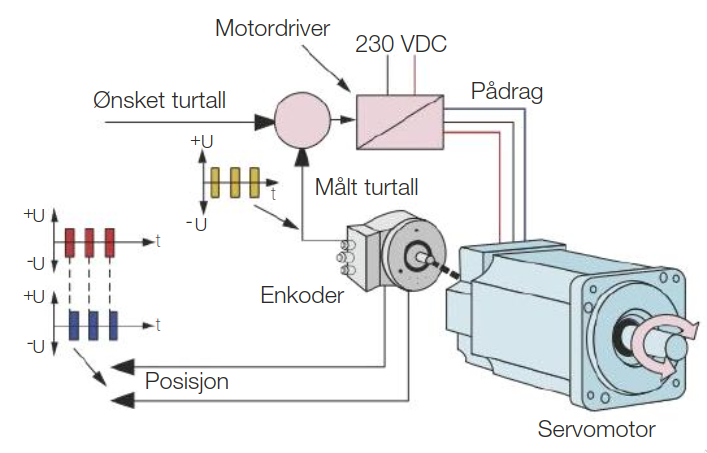
\includegraphics[width=1\textwidth]{../output/nogpl/TurtallPosisjon01.png}$$
		\end{column}
	\end{columns}
\end{frame}

\begin{frame}
	\frametitle{Enkoder i industriell utførelse}
	$$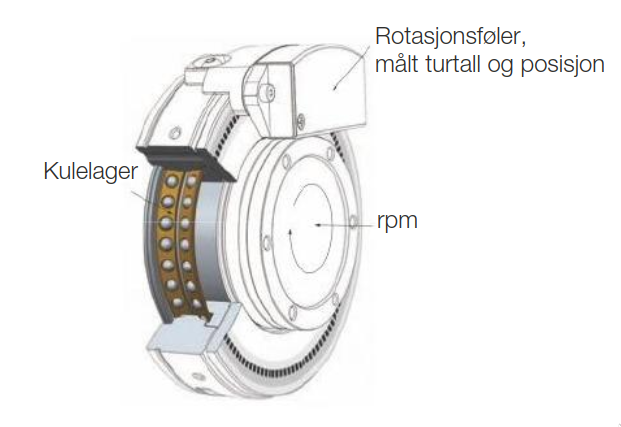
\includegraphics[height=0.8\textheight]{../output/nogpl/TurtallPosisjon02.png}$$
\end{frame}

\begin{frame}
	\frametitle{Kodeskive til bruk i enkodere}
	\begin{columns}
		\begin{column}{0.5\textwidth}
En kodeskive bryter lyset fra en fotodiode til en fototransistor. På denne måten får vi pulser når vi roter på enkoderen. 
			
		\end{column}

		\begin{column}{0.5\textwidth}
	$$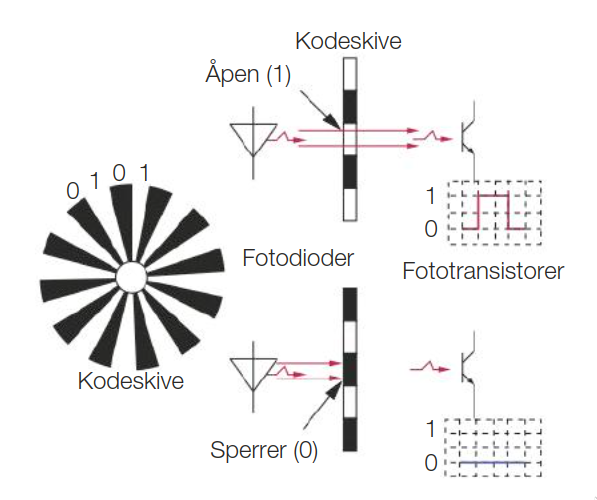
\includegraphics[width=1\textwidth]{../output/nogpl/TurtallPosisjon03.png}$$
		\end{column}
	\end{columns}
\end{frame}

\begin{frame}
	\frametitle{To kodesiver 90° forsøvet}
	\begin{columns}
		\begin{column}{0.5\textwidth}
Ved å bruke to kodesiver kan vi avgjøre hvilken vei enkoderen roterer. 
		\end{column}

		\begin{column}{0.5\textwidth}
	$$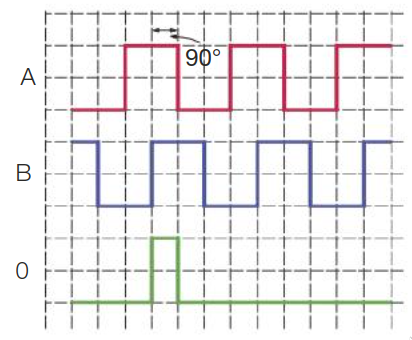
\includegraphics[width=1\textwidth]{../output/nogpl/TurtallPosisjon04.png}$$
		\end{column}
	\end{columns}
\end{frame}

\begin{frame}
	\frametitle{Absolutt giver}
	\begin{columns}
		\begin{column}{0.5\textwidth}
			En absolutt giver har $2^n$ unike posisjoner for hver rotasjon. 
			\vskip 1cm
			Det er vanlig med 8bits absolutt enkoder, denne har $2^8$ posisjoner for en rotasjon. Det gir en oppløsning på $\frac{360^\circ}{256}=1.406^\circ$
			\vskip 1cm
			En 13bits absoluttenkoder vil har en oppløsning på $(2^{13}=8192) \frac{360^\circ}{8192} =0.04394^\circ$
		\end{column}

		\begin{column}{0.5\textwidth}
	$$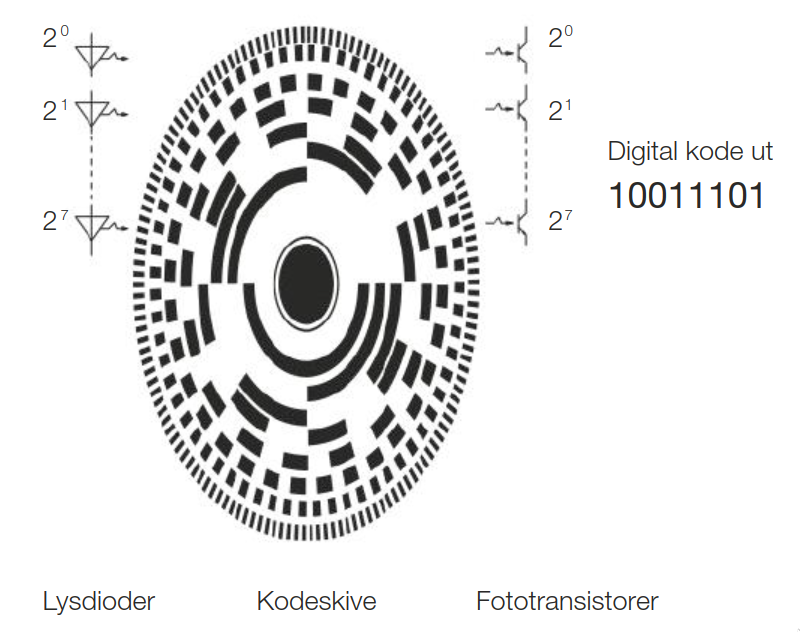
\includegraphics[width=1\textwidth]{../output/nogpl/TurtallPosisjon05.png}$$
		\end{column}
	\end{columns}
\end{frame}

\begin{frame}
	\frametitle{Binærkode}
	\begin{columns}
		\begin{column}{0.5\textwidth}
Ved bruk av binærkode bytter flere bit på samme tid, dette kan gi binærfeil i overgangen mellom posisjonene. Det ideelle hadde vært at bare ett bit byttet om gangen. 
			
		\end{column}

		\begin{column}{0.5\textwidth}
	$$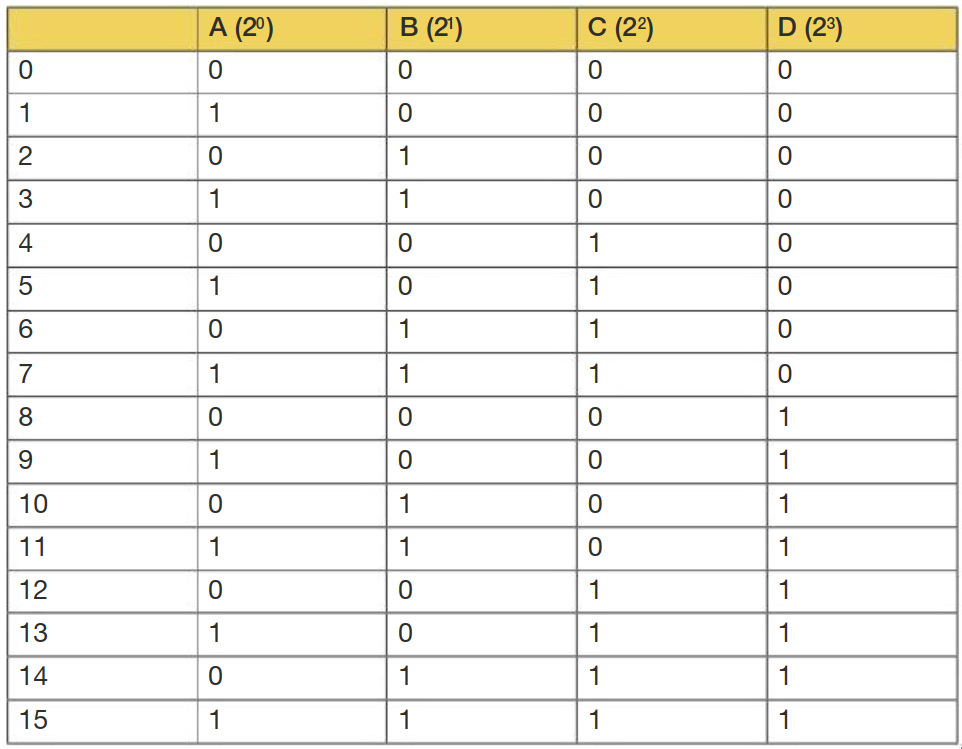
\includegraphics[width=1\textwidth]{../output/nogpl/TurtallPosisjon06.png}$$
		\end{column}
	\end{columns}
\end{frame}

\begin{frame}
	\frametitle{Gray-kode}
	\begin{columns}
		\begin{column}{0.5\textwidth}
Gray-kode tilfredstiller kravet til at bare ett bit skal bytte om gangen. 
			
		\end{column}

		\begin{column}{0.5\textwidth}
	$$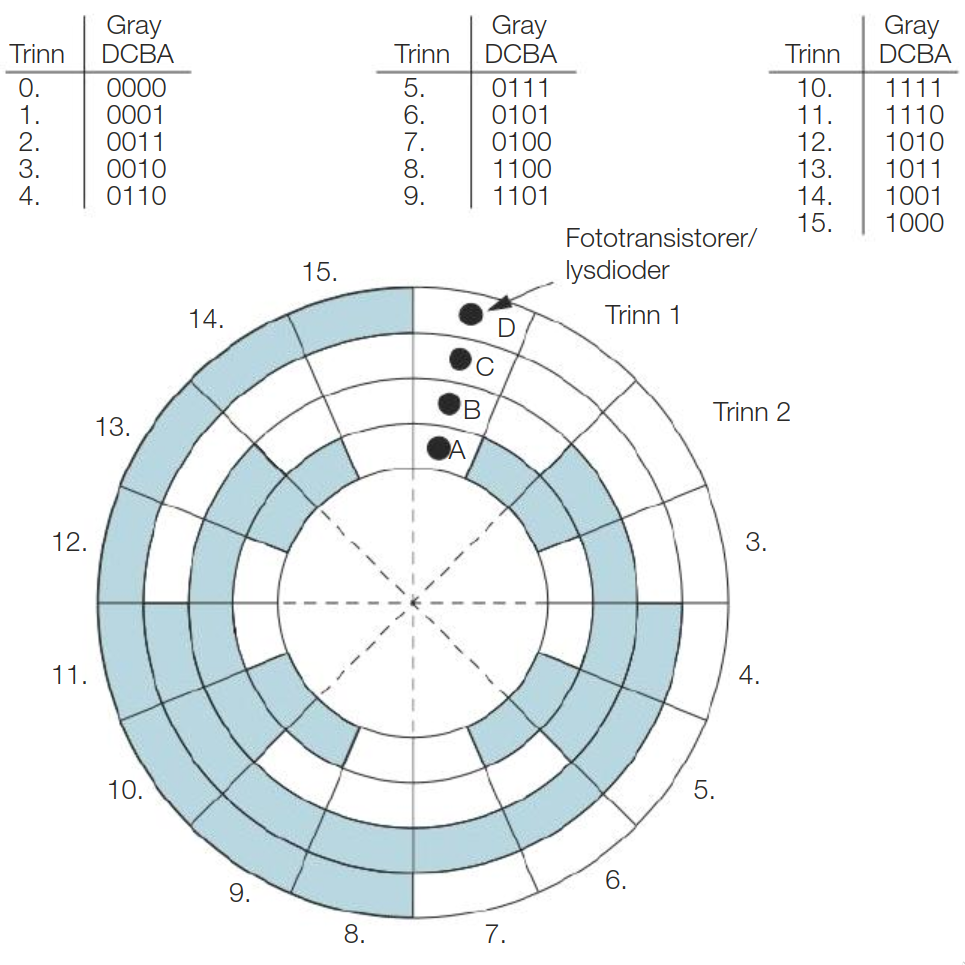
\includegraphics[width=1\textwidth]{../output/nogpl/TurtallPosisjon07.png}$$
		\end{column}
	\end{columns}
\end{frame}

\begin{frame}
	\frametitle{Enkoder med utgang for Gray-kode og binærkode}
	$$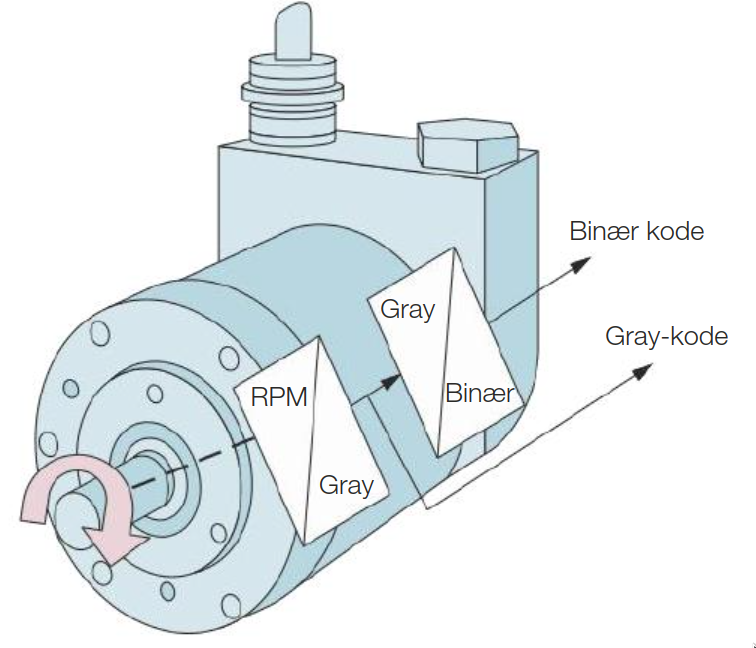
\includegraphics[width=0.5\textwidth]{../output/nogpl/TurtallPosisjon08.png}$$
\end{frame}

\begin{frame}
	\frametitle{Lineærgivere}
	\begin{columns}
		\begin{column}{0.5\textwidth}
Meterstokk
			
		\end{column}

		\begin{column}{0.5\textwidth}
	$$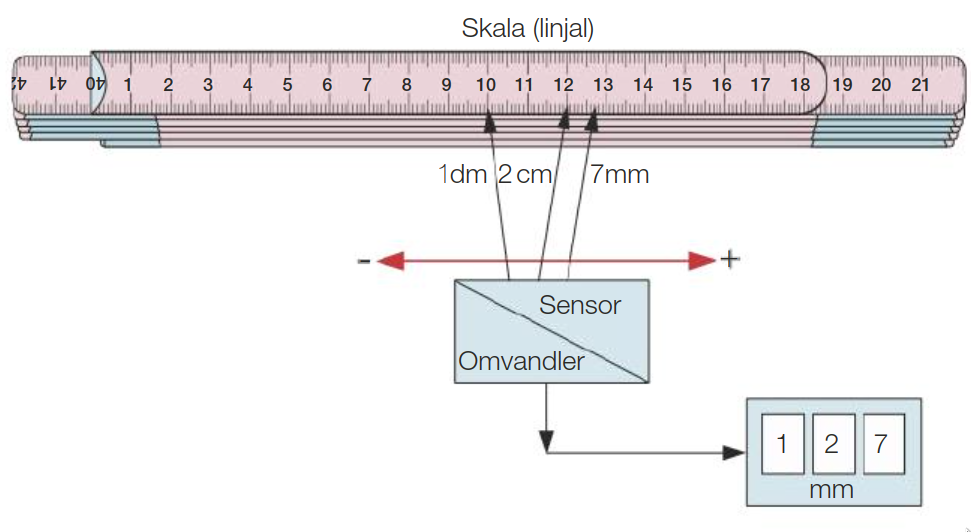
\includegraphics[width=1\textwidth]{../output/nogpl/TurtallPosisjon09.png}$$
		\end{column}
	\end{columns}
\end{frame}

\begin{frame}
	\frametitle{Lineargivere}
	\begin{columns}
		\begin{column}{0.5\textwidth}
Digital målelinjal
\vskip 12pt
Måler vandring langs en rettlinjet bane. Kan ha enmålenøyaktighet på 2µm
	$$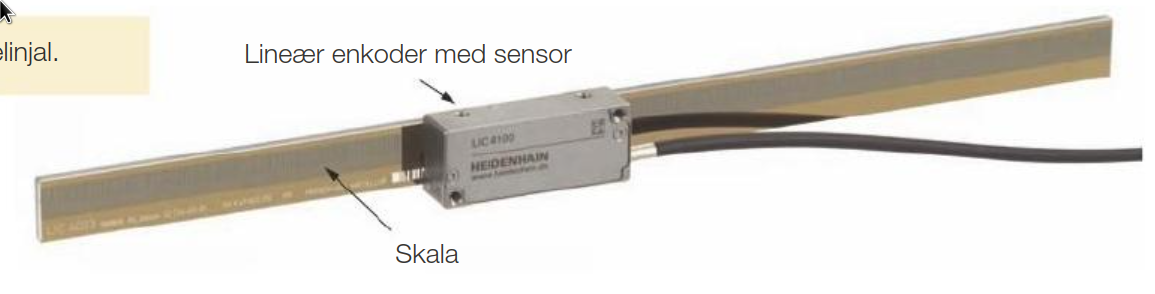
\includegraphics[width=1\textwidth]{../output/nogpl/TurtallPosisjon10.png}$$
			
		\end{column}

		\begin{column}{0.5\textwidth}
	$$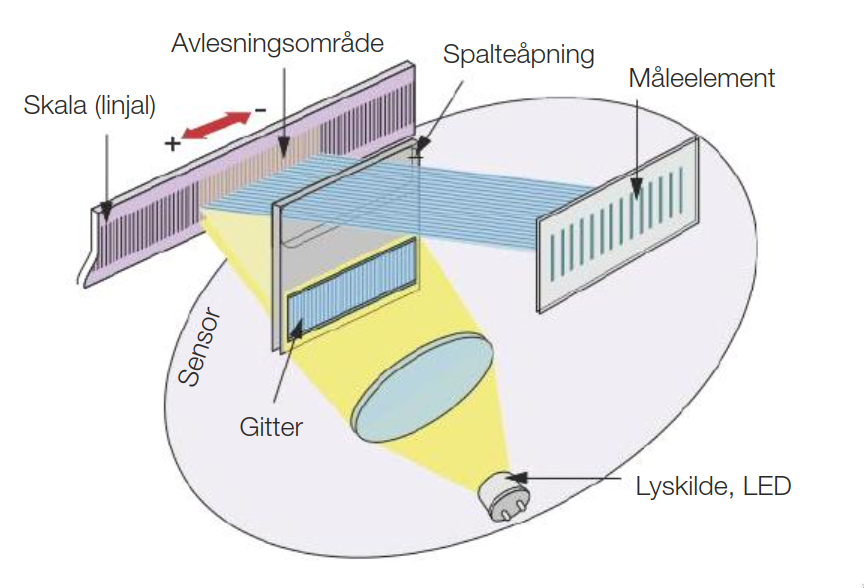
\includegraphics[width=1\textwidth]{../output/nogpl/TurtallPosisjon11.png}$$
		\end{column}
	\end{columns}
\end{frame}


\begin{frame}
	\frametitle{Linelengdegiver}
	\begin{columns}
		\begin{column}{0.5\textwidth}
Fås i utgaver fra 0.2 til 60m. 
			
		\end{column}

		\begin{column}{0.5\textwidth}
	$$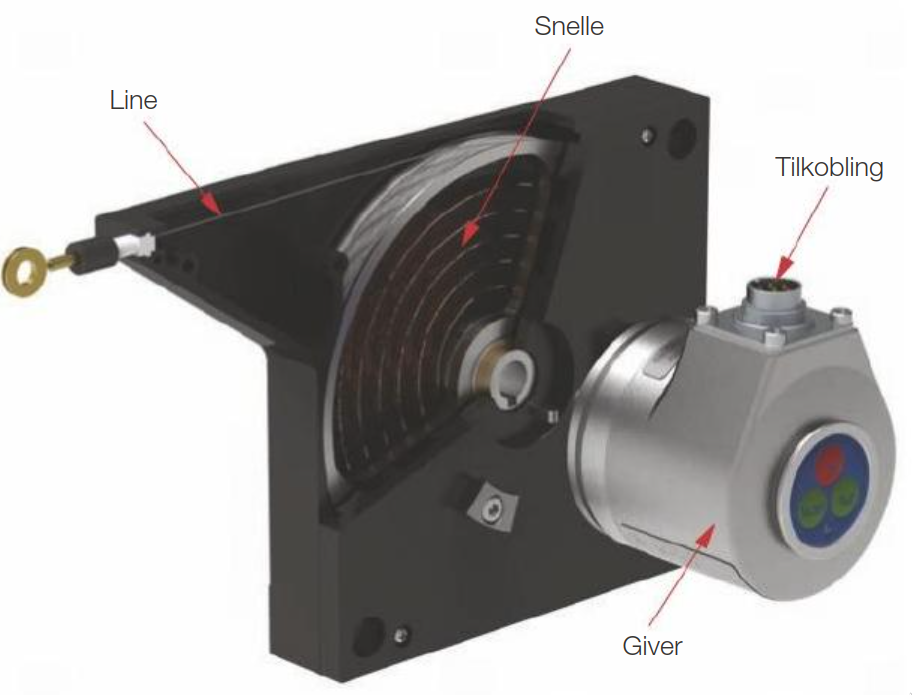
\includegraphics[width=1\textwidth]{../output/nogpl/TurtallPosisjon12.png}$$
		\end{column}
	\end{columns}
\end{frame}

\begin{frame}
	\frametitle{Potensiometer}
	\begin{columns}
		\begin{column}{0.5\textwidth}
Et potensiometer kan kobles til en aksling eller en line som beveger seg i en rettlinje for å angi posisjon.
			
		\end{column}

		\begin{column}{0.5\textwidth}
	$$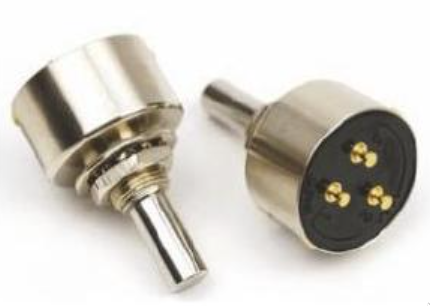
\includegraphics[width=1\textwidth]{../output/nogpl/TurtallPosisjon13.png}$$
		\end{column}
	\end{columns}
\end{frame}

\begin{frame}
	\frametitle{Potensiometer som spenningsdeler}
	\begin{columns}
		\begin{column}{0.5\textwidth}
For å kunne avlese posisjonen brukes potensiometeret som en spenningsdeler. 
			
		\end{column}

		\begin{column}{0.5\textwidth}
	$$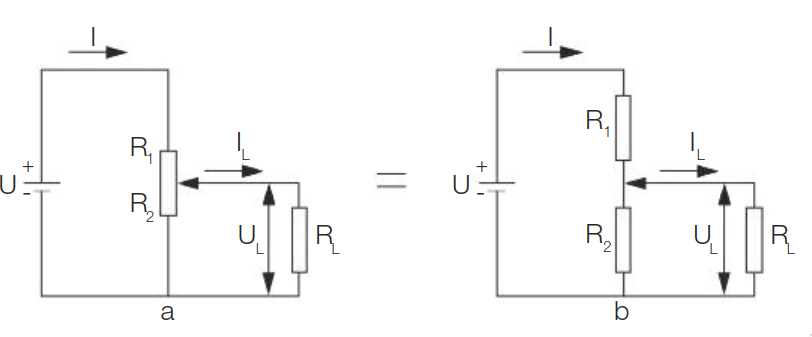
\includegraphics[width=1\textwidth]{../output/nogpl/TurtallPosisjon14.png}$$
		\end{column}
	\end{columns}
\end{frame}

\begin{frame}
	\frametitle{Potensiometer}
	$$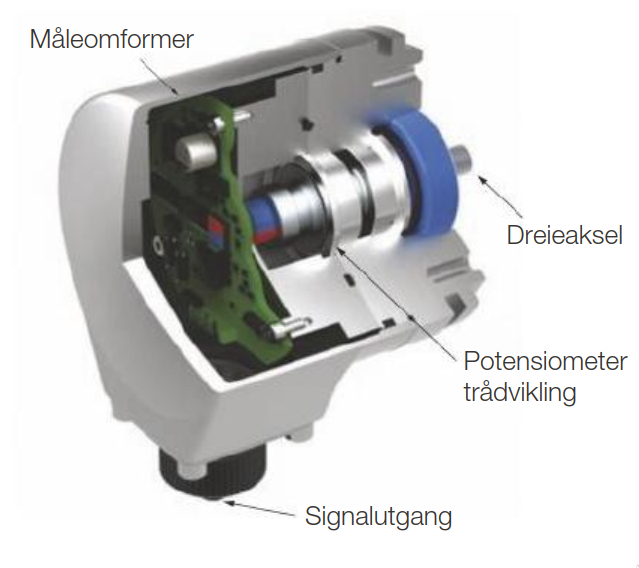
\includegraphics[height=0.8\textheight]{../output/nogpl/TurtallPosisjon15.png}$$
\end{frame}

\begin{frame}
	\frametitle{Potensiometer}
	$$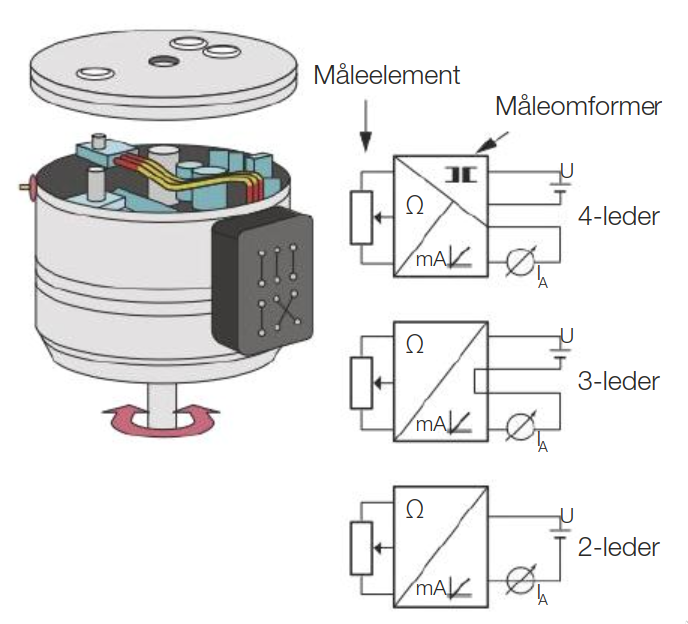
\includegraphics[height=0.8\textheight]{../output/nogpl/TurtallPosisjon16.png}$$
\end{frame}
\begin{frame}
	\frametitle{Potensiometer}
	$$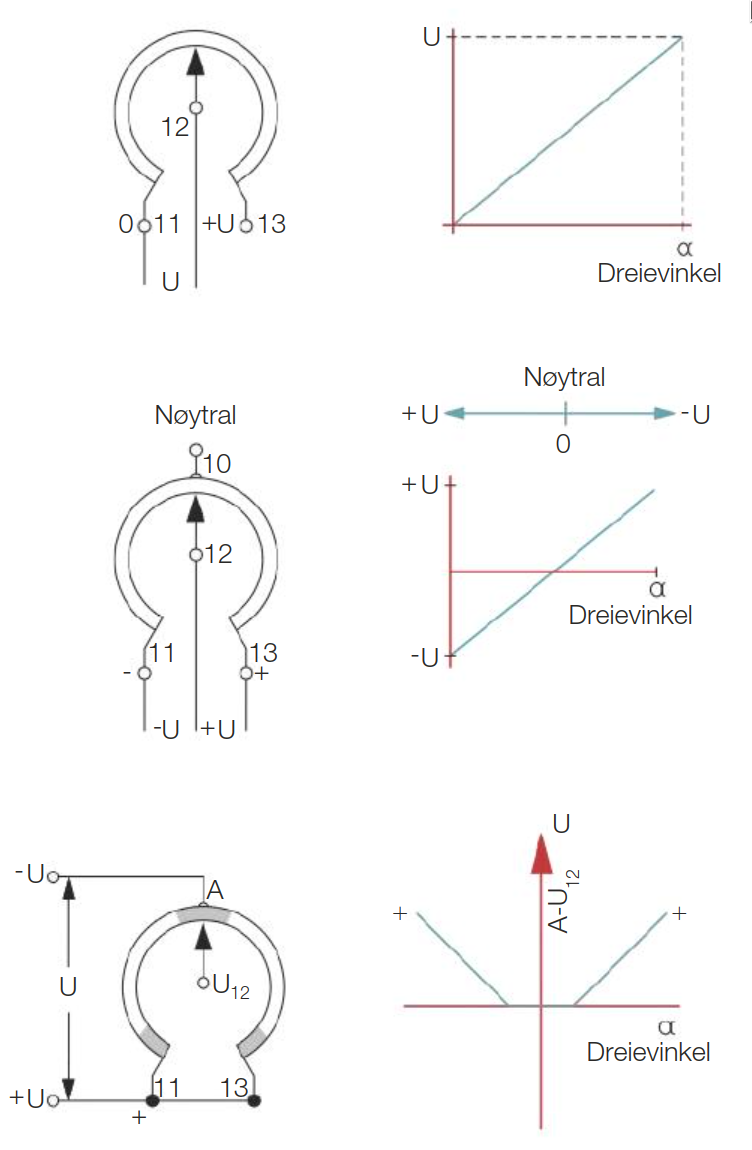
\includegraphics[height=0.8\textheight]{../output/nogpl/TurtallPosisjon17.png}$$
\end{frame}
\begin{frame}
	\frametitle{Lineære potensiomtre}
	$$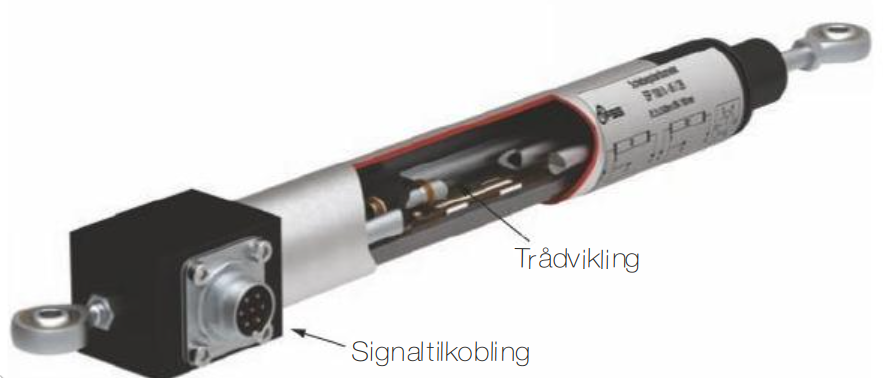
\includegraphics[height=0.7\textheight]{../output/nogpl/TurtallPosisjon18.png}$$
\end{frame}

\end{document}
